\documentclass[aspectratio=169,10pt]{beamer}

\usepackage[utf8]{inputenc}
\usepackage[T1]{fontenc}
\usepackage{lmodern}
\usepackage{xcolor}
\usepackage{pgfplots}
\pgfplotsset{compat=1.17}
\usepackage{amsmath,amssymb}
\usepackage{booktabs}
\usepackage{tikz}
\usetikzlibrary{arrows.meta, positioning, calc, fit, backgrounds}

\definecolor{valen}{RGB}{30,90,170}
\definecolor{valenred}{RGB}{200,60,60}
\definecolor{valengreen}{RGB}{40,140,80}

\newcommand{\R}{\mathbb{R}}
\newcommand{\N}{\mathbb{N}}

\usetheme{Madrid}
\usecolortheme{default}
\setbeamercolor{structure}{fg=valen}
\setbeamertemplate{navigation symbols}{}

\title{Structural Invariants, Attack-Graph Mathematics, and an Autonomous Red-Team Platform}
\author{VALEN Project}
\date{Working draft v0.5}

\begin{document}

\begin{frame}
  \titlepage
\end{frame}

\begin{frame}{Two theses, one typed IR}
  \begin{columns}[T]
    \begin{column}{0.5\textwidth}
      \textbf{Defensive thesis (measured)}\\[2mm]
      \begin{itemize}
        \item Structural invariants (spectral, homology, curvature) add
          \emph{nothing} over taint for injection prioritization.
        \item But they are the \emph{only} signal for authorization (BOLA/IDOR),
          destructive state cycles, and trust topology.
      \end{itemize}
    \end{column}
    \begin{column}{0.5\textwidth}
      \textbf{Offensive thesis}\\[2mm]
      \begin{itemize}
        \item An autonomous red-team platform over the \emph{same} graph.
        \item Differentiator: \emph{quantitative attack-graph mathematics},
          not scripting.
      \end{itemize}
    \end{column}
  \end{columns}
  \vfill
  \centering\small One deterministic typed graph IR $\to$ verifier $\cdot$ planner $\cdot$ platform.
\end{frame}

\begin{frame}{System architecture}
  \centering
  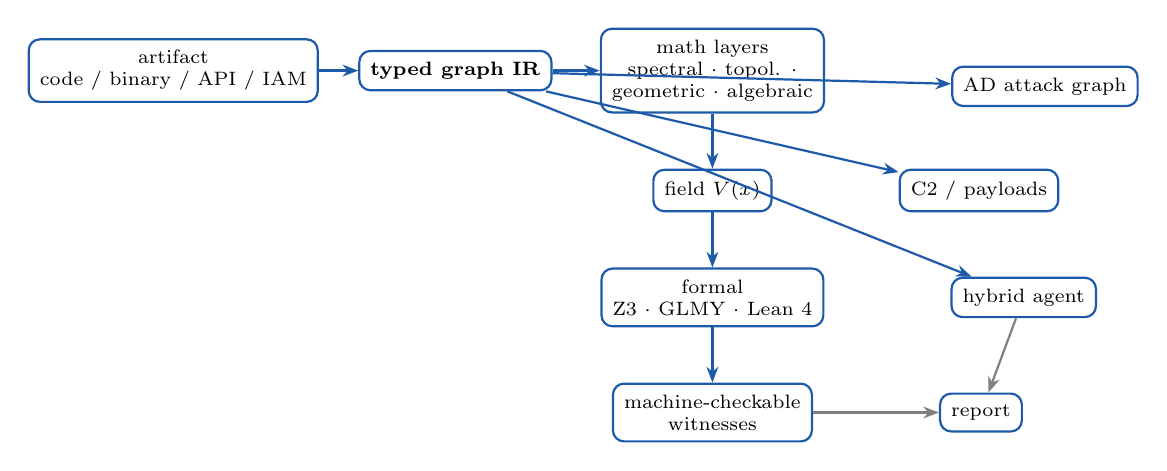
\begin{tikzpicture}[
      box/.style={rectangle, draw=valen, thick, rounded corners, align=center, font=\scriptsize, inner sep=4pt},
      arr/.style={-{Stealth[length=2mm]}, thick, valen},
    ]
    \node[box] (art) {artifact\\code / binary / API / IAM};
    \node[box, right=5mm of art] (ir) {\textbf{typed graph IR}};
    \node[box, right=6mm of ir] (layers) {math layers\\spectral $\cdot$ topol. $\cdot$\\geometric $\cdot$ algebraic};
    \node[box, below=7mm of layers] (field) {field $V(x)$};
    \node[box, below=7mm of field] (verify) {formal\\Z3 $\cdot$ GLMY $\cdot$ Lean 4};
    \node[box, below=7mm of verify] (wit) {machine-checkable\\witnesses};
    \node[box, right=16mm of layers, yshift=-2mm] (ad) {AD attack graph};
    \node[box, right=16mm of field] (c2) {C2 / payloads};
    \node[box, right=16mm of verify] (agent) {hybrid agent};
    \node[box, right=16mm of wit] (report) {report};
    \draw[arr] (art) -- (ir); \draw[arr] (ir) -- (layers);
    \draw[arr] (layers) -- (field); \draw[arr] (field) -- (verify);
    \draw[arr] (verify) -- (wit);
    \draw[arr] (ir) -- (ad); \draw[arr] (ir) -- (c2);
    \draw[arr] (ir) -- (agent); \draw[arr, gray] (agent) -- (report);
    \draw[arr, gray] (wit) -- (report);
  \end{tikzpicture}
\end{frame}

\begin{frame}{The boundary result (injection SAST)}
  \centering
  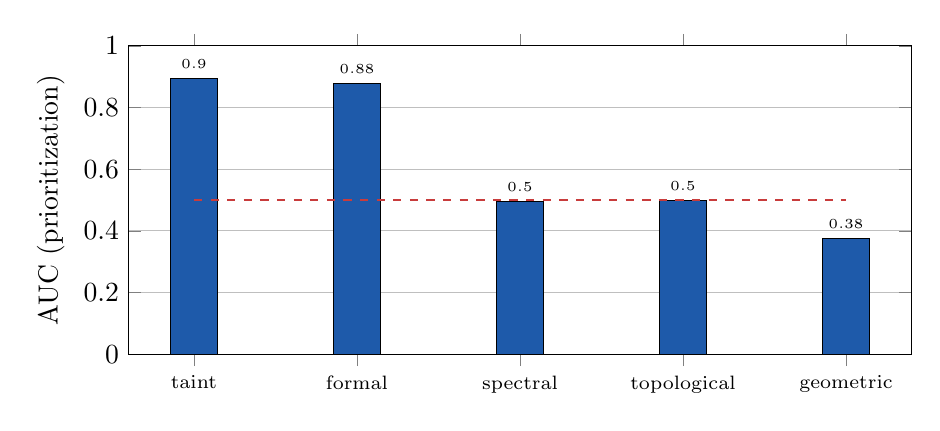
\begin{tikzpicture}
    \begin{axis}[
        ybar, bar width=0.6cm, width=0.95\linewidth, height=5.5cm,
        symbolic x coords={taint, formal, spectral, topological, geometric},
        xtick=data, x tick label style={font=\scriptsize},
        ymin=0, ymax=1.0, ylabel={AUC (prioritization)},
        nodes near coords, every node near coord/.append style={font=\tiny},
        ymajorgrids=true,
      ]
      \addplot[fill=valen] coordinates {
        (taint,0.895) (formal,0.878) (spectral,0.496)
        (topological,0.500) (geometric,0.376)};
      \draw[dashed, valenred, thick] (axis cs:taint,0.5) -- (axis cs:geometric,0.5);
    \end{axis}
  \end{tikzpicture}
  \begin{itemize}\small
    \item OWASP Benchmark~1.2 (2740 cases): taint MRR $0.894$ beats fused field $0.872$ ($p=5\times10^{-5}$).
    \item Spectral/topological at chance; curvature below chance. \emph{A falsifiable negative result.}
  \end{itemize}
\end{frame}

\begin{frame}{Authorization, mechanized and operational}
  \begin{itemize}\small
    \item Privilege-level function $F:V\to\N$; auth edge iff $F(u)<F(v)$; \texttt{no\_auth\_bounded} mechanized in Lean~4.
    \item Structural BOLA/IDOR detector: recall $1.0$ / precision $0.72$ / F1 $0.837$ where taint scores $0$.
    \item Z3 ownership witness $\mathrm{SAT}(\mathrm{owner}(id)\ne session)$: separates object-level authorization from mere authentication.
    \item Real data (crAPI, 9 endpoints): recall $1.0$ / precision $0.90$; the missing-auth check scores $0$ because BOLA \emph{is} authenticated.
  \end{itemize}
  \centering
  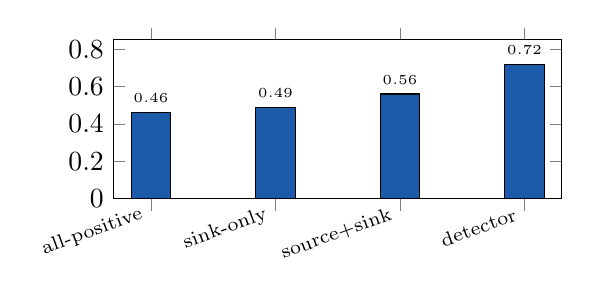
\begin{tikzpicture}
    \begin{axis}[ybar, bar width=0.5cm, width=0.6\linewidth, height=3.6cm,
        symbolic x coords={all-positive, sink-only, source+sink, detector},
        xtick=data, x tick label style={rotate=20, anchor=east, font=\scriptsize},
        ymin=0, ymax=0.85, nodes near coords, every node near coord/.append style={font=\tiny}]
      \addplot[fill=valen] coordinates {(all-positive,0.46)(sink-only,0.49)(source+sink,0.56)(detector,0.72)};
    \end{axis}
  \end{tikzpicture}
\end{frame}

\begin{frame}{Directed path homology (GLMY)}
  \centering
  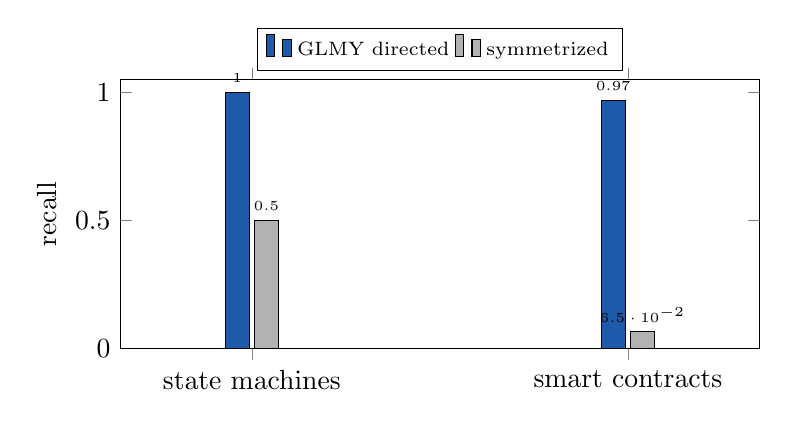
\begin{tikzpicture}
    \begin{axis}[ybar, bar width=0.3cm, width=0.8\linewidth, height=5cm,
        symbolic x coords={state machines, smart contracts}, xtick=data,
        ymin=0, ymax=1.05, ylabel={recall},
        legend style={at={(0.5,1.03)}, anchor=south, legend columns=-1, font=\scriptsize},
        nodes near coords, every node near coord/.append style={font=\tiny}, enlarge x limits=0.35]
      \addplot[fill=valen] coordinates {(state machines,1.00)(smart contracts,0.968)};
      \addplot[fill=gray!60] coordinates {(state machines,0.50)(smart contracts,0.065)};
      \legend{GLMY directed, symmetrized}
    \end{axis}
  \end{tikzpicture}
  \begin{itemize}\small
    \item Symmetrization collapses the directed 2-cycle: recall $1.0\to0.5$ (state), $0.97\to0.065$ (contracts).
    \item Returns the concrete $\beta_1$ generator as evidence.
  \end{itemize}
\end{frame}

\begin{frame}{Multi-language SAST}
  \centering
  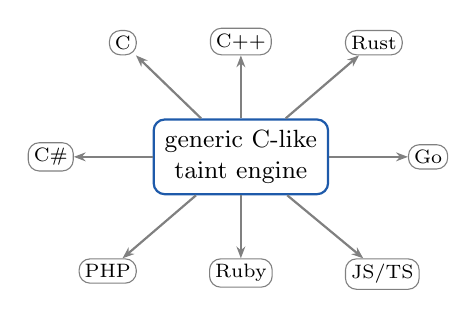
\begin{tikzpicture}[
      box/.style={rectangle, draw=valen, thick, rounded corners, align=center, font=\small, inner sep=4pt},
      lang/.style={rectangle, draw=gray, rounded corners, align=center, font=\scriptsize, inner sep=2pt},
      arr/.style={-{Stealth[length=1.5mm]}, gray, thick}]
    \node[box] (e) {generic C-like\\taint engine};
    \node[lang, above left=8mm and 2mm of e] (c) {C};
    \node[lang, above=8mm of e] (cpp) {C++};
    \node[lang, above right=8mm and 2mm of e] (rust) {Rust};
    \node[lang, left=10mm of e] (cs) {C\#};
    \node[lang, right=10mm of e] (go) {Go};
    \node[lang, below left=8mm and 2mm of e] (php) {PHP};
    \node[lang, below=8mm of e] (ruby) {Ruby};
    \node[lang, below right=8mm and 2mm of e] (js) {JS/TS};
    \draw[arr] (e)--(c); \draw[arr] (e)--(cpp); \draw[arr] (e)--(rust);
    \draw[arr] (e)--(cs); \draw[arr] (e)--(go); \draw[arr] (e)--(php);
    \draw[arr] (e)--(ruby); \draw[arr] (e)--(js);
  \end{tikzpicture}
  \begin{itemize}\small
    \item 9 grammars, 1 engine; per-language source/sink/sanitizer profiles.
    \item Canonical \texttt{categories.py}: severity + CWE + OWASP + CVSS 3.1/4.0 + MITRE per finding.
  \end{itemize}
\end{frame}

\begin{frame}{The red-team platform}
  \centering
  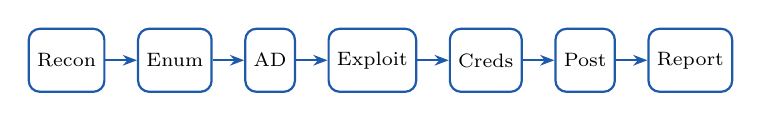
\begin{tikzpicture}[
      box/.style={rectangle, draw=valen, thick, rounded corners, align=center, font=\scriptsize, inner sep=3pt, minimum height=8mm},
      arr/.style={-{Stealth[length=1.8mm]}, thick, valen}]
    \node[box] (a) {Recon}; \node[box, right=4mm of a] (b) {Enum};
    \node[box, right=4mm of b] (c) {AD}; \node[box, right=4mm of c] (d) {Exploit};
    \node[box, right=4mm of d] (e) {Creds}; \node[box, right=4mm of e] (f) {Post};
    \node[box, right=4mm of f] (g) {Report};
    \draw[arr] (a)--(b); \draw[arr] (b)--(c); \draw[arr] (c)--(d);
    \draw[arr] (d)--(e); \draw[arr] (e)--(f); \draw[arr] (f)--(g);
  \end{tikzpicture}
  \begin{itemize}\small
    \item Multi-user \emph{team server}: roles (viewer/operator/admin), PBKDF2 sessions, RBAC, SSE live collaboration, SQLite persistence.
    \item Recon $\to$ AD $\to$ C2/payloads $\to$ creds (Kerberoast/PCFG) $\to$ phishing/exfil $\to$ report.
    \item \emph{Authorization-first}: scope allow-list, \texttt{--allow-exec}, operator approval.
  \end{itemize}
\end{frame}

\begin{frame}{Attack-graph mathematics}
  \centering
  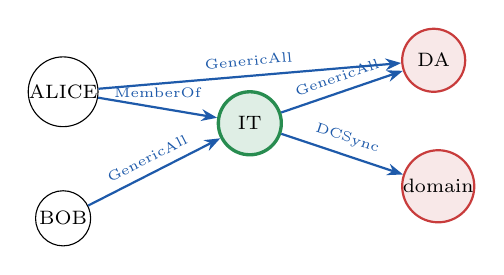
\begin{tikzpicture}[
      n/.style={circle, draw, inner sep=0pt, minimum size=7mm, font=\scriptsize, align=center},
      target/.style={circle, draw=valenred, thick, fill=valenred!12, inner sep=0pt, minimum size=8mm, font=\scriptsize, align=center},
      chok/.style={circle, draw=valengreen, very thick, fill=valengreen!15, inner sep=0pt, minimum size=8mm, font=\scriptsize, align=center},
      arr/.style={-{Stealth[length=2mm]}, thick, valen, font=\tiny}]
    \node[n] (alice) {ALICE}; \node[n, below=8mm of alice] (bob) {BOB};
    \node[chok, right=15mm of alice, yshift=-4mm] (it) {IT};
    \node[target, right=15mm of it, yshift=8mm] (da) {DA};
    \node[target, right=15mm of it, yshift=-8mm] (dom) {domain};
    \draw[arr] (alice) -- node[above, sloped]{GenericAll} (da);
    \draw[arr] (alice) -- node[above]{MemberOf} (it);
    \draw[arr] (bob) -- node[above, sloped]{GenericAll} (it);
    \draw[arr] (it) -- node[above, sloped]{GenericAll} (da);
    \draw[arr] (it) -- node[above, sloped]{DCSync} (dom);
  \end{tikzpicture}
  \begin{itemize}\small
    \item \textbf{Min-cut (Menger)}: chokepoints (BOB$\to$IT, min-cut 1).
    \item \textbf{Min-cost flow}: cheapest disjoint plans. \textbf{Hitting probability}: exact $(I-Q)^{-1}R$.
    \item \textbf{Z3 synthesis}: minimal-cost ordered exploit plans + AND-preconditions.
    \item \textbf{PCFG}: probabilistic password prior from a cracked corpus.
  \end{itemize}
\end{frame}

\begin{frame}{Evaluation}
  \begin{columns}[T]
    \begin{column}{0.5\textwidth}
      \textbf{Autonomous pentest (crAPI)}\\[2mm]
      
\begin{tikzpicture}
        \draw[gray!30, line width=8pt] (0,0) -- (6,0);
        \draw[valengreen, line width=8pt] (0,0) -- (6,0);
        \node[above, font=\scriptsize] at (3,0.15) {18/18};
      \end{tikzpicture}
      \begin{itemize}\scriptsize
        \item BOLA/BFLA, mass assignment, SSRF, NoSQL/SQLi, JWT, LLM prompt injection.
        \item BOLA recall 1.0 / precision 0.90.
      \end{itemize}
    \end{column}
    \begin{column}{0.5\textwidth}
      \textbf{Results at a glance}\\[1mm]
      {\scriptsize
      \begin{tabular}{@{}ll@{}}
        \toprule
        boundary & taint $0.894$ vs field $0.872$ \\
        BOLA/IDOR & $1.0$ / $0.90$ (crAPI) \\
        GLMY & $0.97$ vs $0.065$ recall \\
        arbitration & agreement $0.974$ \\
        languages & 9, 1 engine \\
        tests & 383 green \\
        \bottomrule
      \end{tabular}}
    \end{column}
  \end{columns}
\end{frame}

\begin{frame}{Conclusion}
  \begin{itemize}
    \item \textbf{Defensive}: structural invariants verify authorization, state, and trust --- not injection prioritization (measured boundary).
    \item \textbf{Offensive}: a red-team platform whose differentiator is \emph{quantitative attack-graph mathematics}.
    \item \textbf{One typed IR} joins both; every result carries a machine-checkable witness.
    \item Installable, tested, documented; authorization-first by design.
  \end{itemize}
\end{frame}

\end{document}
